\documentclass[10pt]{article}

\usepackage[T1]{fontenc}
\usepackage[utf8]{inputenc}
%\usepackage{beton}
%\usepackage{ccfonts}
%\usepackage{concrete}
\usepackage{concmath}
\usepackage{eulervm}
\usepackage{amsmath,amsthm,amssymb}
\usepackage{mathtools}
\usepackage{multicol}
\usepackage{marginnote}
\usepackage{pgfplots}
\usepackage{float}
\usepackage{hyperref}
\pgfplotsset{compat=1.5}

\usepackage{mathtools}

\usepackage{wasysym}
\usepackage[margin=1.5in]{geometry} 
\usepackage{enumerate}
\index{\usepackage}\usepackage{multicol}

\newcommand{\N}{\mathbf{N}}
\newcommand{\Z}{\mathbb{Z}}

\newcommand{\R}{\mathbf{R}}
\newcommand{\C}{\mathbf{C}}
\newcommand{\Pbb}{\mathbb{P}}
\newcommand{\Fcal}{\mathcal{F}}
\newcommand{\Acal}{\mathcal{A}}
\newcommand{\Ecal}{\mathcal{E}}
\newcommand{\Ebb}{\mathbb{E}}
\newcommand{\Qbb}{\mathbb{Q}}

\newenvironment{theorem}[2][Theorem]{\begin{trivlist}
  \item[\hskip \labelsep {\bfseries #1}\hskip \labelsep {\bfseries #2.}]}{\end{trivlist}}
\newenvironment{lemma}[2][Lemma]{\begin{trivlist}
  \item[\hskip \labelsep {\bfseries #1}\hskip \labelsep {\bfseries #2.}]}{\end{trivlist}}
\newenvironment{exercise}[2][Exercise]{\begin{trivlist}
  \item[\hskip \labelsep {\bfseries #1}\hskip \labelsep {\bfseries #2.}]}{\end{trivlist}}
\newenvironment{reflection}[2][Reflection]{\begin{trivlist}
  \item[\hskip \labelsep {\bfseries #1}\hskip \labelsep {\bfseries #2.}]}{\end{trivlist}}
\newenvironment{proposition}[2][Proposition]{\begin{trivlist}
  \item[\hskip \labelsep {\bfseries #1}\hskip \labelsep {\bfseries #2.}]}{\end{trivlist}}
\newenvironment{corollary}[2][Corollary]{\begin{trivlist}
  \item[\hskip \labelsep {\bfseries #1}\hskip \labelsep {\bfseries #2.}]}{\end{trivlist}}

\newenvironment{definition}[2][Definition]{\begin{trivlist}
  \item[\hskip \labelsep {\bfseries #1}\hskip \labelsep {\bfseries #2.}]}{\end{trivlist}}

\begin{document}
	
  \renewcommand{\qedsymbol}{\smiley}
	\title{Investments Class \\ Problem set 1}
	\author{Daniel Grosu, William Martin, Denis Steffen}
	
	\maketitle

  \begin{exercise}{1}
    First, we need to solve the Geometric Brownian Motion SDE. 
    The SDE is given by: 
    $$ \frac{dS_t}{S_t} = \mu dt + \sigma dz_t$$ where $z_t$ is a standard Brownian Motion. 
    We can apply Itô's lemma on the stochastic process $Y_t = f(S_t) = \ln(S_t)$.
    Thus, $$ dY_t = 0 dt +  \frac{1}{S_t}dS_t + \frac{1}{2}\frac{-1}{S_t^2}(\sigma S_t)^2 dt = \mu dt + \sigma dz_t - \frac{\sigma^2}{2}dt$$
    and $$ \ln(S_t) = (\mu-\frac{\sigma^2}{2})t + \sigma dz_t$$
    The solution of the SDE is: $ S_t = S_0 \exp((\mu-\frac{\sigma^2}{2})t+ \sigma z_t)$.
    Simulating on $10$ years, with the given drift and volatility parameters, the share price can be found in Figure \ref{GMB}. The corresponding log-returns of the share are displayed in Figure \ref{DLR}.
    With this data, we can compute the annualized mean and standard deviation of log-returns:
    
    \begin{table}[h]
      \centering
        \begin{tabular}{|l|l|}
        \hline
        Annualized mean & Annualized Standard Deviation \\ \hline
        7.659 \%        & 20.336 \%                    \\ \hline
        \end{tabular}
        \caption{Simulation log-returns statistics}
      \end{table}
      We can see that the estimators of simulated share prices are consistent with the parameters $\mu = 6\%$ and $\sigma = 20\%$ but there is still high variance in the estimation. 

  \begin{figure}[h]
	\centering
	\begin{minipage}[b]{0.49\textwidth}
		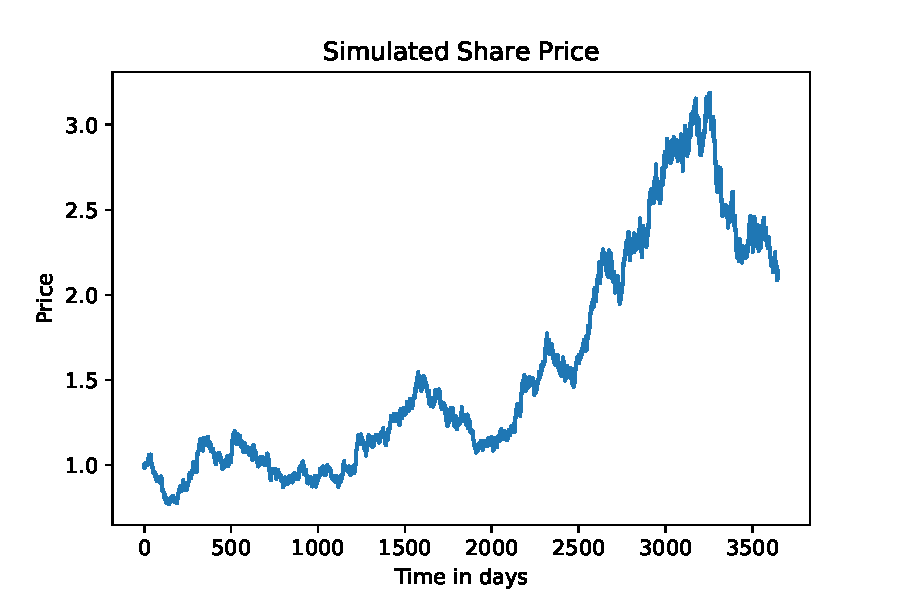
\includegraphics[width = \textwidth]{Figures/simulation.pdf}
		\caption{Share price simulation}
		\label{GMB}
	\end{minipage}
	\hfill
	\begin{minipage}[b]{0.49\textwidth}
		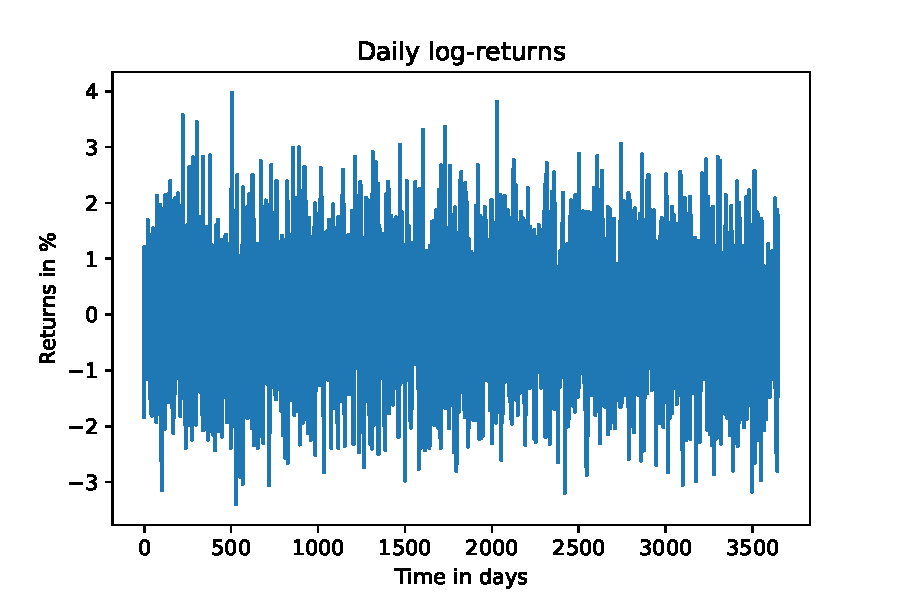
\includegraphics[width = \textwidth]{Figures/logreturns.pdf}
		\caption{Daily log-returns}
		\label{DLR}
  \end{minipage}	
  \end{figure}
  \end{exercise}

  \begin{exercise}{2}
    To control the accuracy of our estimators of the mean and the volatility, we can simulate more samples and estimate the variance of these two estimators.
    We have simulated daily share prices from January $1^{\text{st}}$, $1950$ to December $31^{\text{st}}$, 2018 and so we get $25202$ daily samples. We can resample the daily prices into monthly ones by taking local monthly averages. The graph of the daily and averaged monthly share prices are in Figures \ref{GMB2} and \ref{GMB2M}.
    \begin{figure}[h]
      \centering
      \begin{minipage}[b]{0.49\textwidth}
        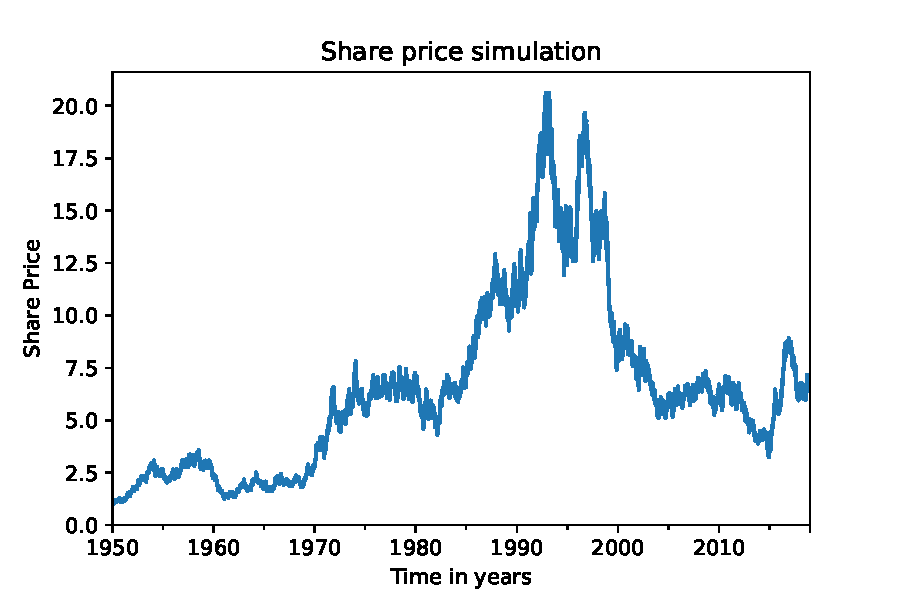
\includegraphics[width = \textwidth]{Figures/simulation2.pdf}
        \caption{Share price simulation (daily)}
        \label{GMB2}
      \end{minipage}
      \hfill
      \begin{minipage}[b]{0.49\textwidth}
        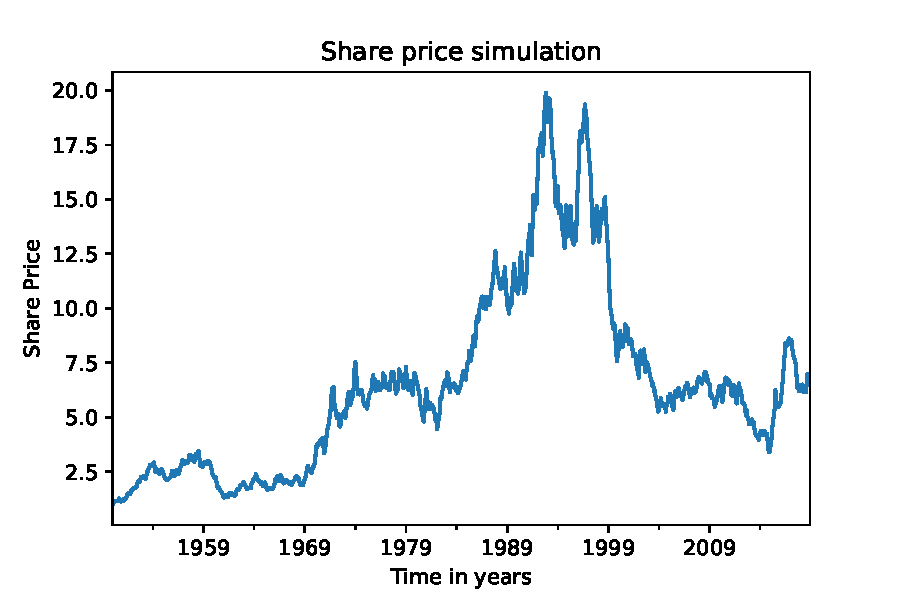
\includegraphics[width = \textwidth]{Figures/simulation2monthly.pdf}
        \caption{Monthly average}
        \label{GMB2M}
      \end{minipage}	
      \end{figure}
  \end{exercise}


  %\section*{Python Code}

  % \subsection*{Exercise}
  % \lstinputlisting{code/exercise.py}
\end{document}
 